\chapter{A WaccApp frontend architektúrája és mappaszerkezete}

A korábbi fejezetek bemutatták, hogy a WaccApp frontendje több, egymást kiegészítő felhasználói folyamat köré szerveződik. Ebben a fejezetben már nem a tervezési indoklás vagy a használhatósági háttér áll a középpontban, hanem a konkrét frontendarchitektúra: mely nézetekből, fájlokból és mappákból épül fel a rendszer, és ezek hogyan kapcsolódnak egymáshoz.

A fejezet célja annak bemutatása, hogy a WaccApp saját fájlszerkezete és nézetrendszere hogyan támogatja a megvalósított funkciókat. Itt kap helyet a fő HTML-nézetek felelőssége, a kliensoldali adatáramlás konkrétabb értelmezése, a nézetek közötti kapcsolat, valamint a frontend szempontból fontos mappák és állományok szerepe.

\section{A többnézetes frontend szervezési logikája}

A WaccApp frontendje több belépőpontos webes felületként épül fel. A gyakorlatban ez azt jelenti, hogy a fő funkciók külön HTML-oldalakhoz kapcsolódnak, de közös kommunikációs adatokat, hasonló felületi mintákat és azonos backendkapcsolatokat használnak. Ebben a fejezetben a hangsúly már nem a többnézetes döntés indoklásán, hanem az egyes nézetek felelősségi körén és kapcsolódásán van.

A többnézetes szervezés ezért a WaccApp-ban nem az oldalak véletlenszerű szétválasztását jelenti, hanem a feladatok felelősségi körök szerinti elkülönítését. Az \path{index.html} a küldési műveletek központi indítófelületeként működik. A kommunikáció visszakövetését a \path{messages.html}, a \path{sent-messages.html} és a \path{conv.html} támogatja. A kérdőíves és sablonos szerkesztési feladatok a \path{questionnaire.html}, a \path{template.html}, a \path{template-menu.html} és a \path{template-single.html} oldalakhoz kapcsolódnak. A \path{filter.html} önálló elemző és visszakereső nézetként jelenik meg, míg a \path{login.html}, a \path{menu.html}, az \path{admin.html}, az \path{account.html} és a \path{privacy.html} a hozzáféréshez, navigációhoz, adminisztrációhoz és tájékoztatáshoz kötődő feladatokat fedik le. 

Ez a szervezési logika azért előnyös, mert minden oldal egy elsődleges feladatra koncentrálhat. Az \path{index.html} nem terhelődik túl részletes statisztikai vagy adminisztratív elemekkel, mert ezek más nézetek felelősségi körébe tartoznak. A \path{filter.html} nem küldési felületként működik, hanem a már létrejött kommunikációs adatok értelmezésére szolgál. A \path{conv.html} nem általános üzenetlista, hanem egy adott kontakthoz kapcsolódó beszélgetés követését támogatja. Így a frontend szerkezete nemcsak fejlesztői oldalról válik átláthatóbbá, hanem a felhasználó számára is könnyebben tanulható rendszert eredményez. 

A WaccApp ebben az értelemben nem klasszikus egyoldalas alkalmazásként működik, de nem is egyszerű, egymástól elszigetelt HTML-oldalak gyűjteménye. Az egyes nézetek közös backendkapcsolatokon, azonos kommunikációs adatokon és hasonló felhasználói mintákon keresztül kapcsolódnak egymáshoz. A rendszer szerkezeti logikája tehát az elkülönítés és az összekapcsolás egyensúlyára épül. 

\section{A fő frontend nézetek felelőssége}

A WaccApp frontendjének egyik legfontosabb nézete az \path{index.html}, amely a kommunikációs műveletek központi indítófelülete. Ezen az oldalon találkozik a felhasználó azokkal a fő műveletekkel, amelyekkel üzenetet, sablont, kérdőívet vagy médiafájlt küldhet, illetve időzített küldést állíthat be. Az oldal felelőssége ezért nem egyszerűen egy üzenetmező megjelenítése, hanem több küldési mód egy felületen belüli kezelése. A frontendnek ebben a nézetben a választott művelethez igazodva kell kezelnie a beviteli mezőket, a szükséges adatokat és a művelet indítását. 

A \path{messages.html} és a \path{sent-messages.html} a kommunikációs események listaalapú visszakövetését támogatják. A két nézet szerepe abban különíthető el, hogy a beérkező és az elküldött tartalmak nem keverednek egyetlen túlterhelt listába, hanem célzottan áttekinthetők. Ez a felosztás akkor válik különösen hasznossá, amikor a felhasználó nem egy konkrét beszélgetést szeretne megnyitni, hanem gyorsan ellenőrizni akarja, milyen üzenetek érkeztek be, vagy milyen tartalmak kerültek korábban elküldésre. 

A \path{conv.html} a kommunikáció részletesebb értelmezésére szolgál. Ez a nézet egy adott kontakthoz kapcsolódó beszélgetésfolyamot jelenít meg, ezért más felületi logikát igényel, mint egy egyszerű listaoldal. A beszélgetésnézetben az időrendiség, a bejövő és kimenő üzenetek elkülönítése, valamint a szöveges és médiás tartalmak értelmezhető megjelenítése kerül előtérbe. A \path{conv.html} jelentősége abban áll, hogy a korábbi kommunikációt nem darabokra bontott adatsorként, hanem folyamatként mutatja meg. 

A \path{filter.html} a visszakeresés és az alapvető értelmezés nézete. Ez az oldal nem új kommunikációs műveletet indít, hanem a már meglévő adatokból segít célzott eredményeket előállítani. A felhasználó név, telefonszám, üzenettípus, dátumintervallum, kérdőív vagy válasz alapján szűrhet, ezért a nézet felelőssége túlmutat egy egyszerű keresőmezőn. A \path{filter.html} feladata az, hogy a több feltételből álló keresést kezelhető formába rendezze, és az eredményeket a felhasználó számára áttekinthetően jelenítse meg. 

A kérdőíves működéshez két eltérő logikájú szerkesztői irány kapcsolódik. A \path{questionnaire.html} a szöveges vagy számalapú válaszokra épülő kérdőívek kezelését támogatja, ahol a kérdések, válaszok és elágazások szerkesztése a fő feladat. Ezzel szemben a \path{template.html}, a \path{template-menu.html} és a \path{template-single.html} a sablonos, gombos kommunikációhoz kapcsolódó szerkesztési felületeket adják. A \path{template-menu.html} navigációs szerepet kap a sablonos feladatok között, a \path{template-single.html} az egyszerűbb sablonkészítési folyamatot támogatja, míg a \path{template.html} az összetettebb, több lépésből álló sablonos kérdőívlogika szerkesztéséhez kapcsolódik. 

A belépési és kiegészítő nézetek szintén a frontend egészének részei, de más szerepet töltenek be, mint a kommunikációs modulok. A \path{login.html} a belépési folyamatot biztosítja, a \path{menu.html} a főbb oldalak közötti navigációt segíti, az \path{admin.html} az adminisztratív feladatokhoz kapcsolódik, az \path{account.html} a felhasználói fiókhoz tartozó beállítások nézete, a \path{privacy.html} pedig az adatvédelmi tájékoztatás megjelenítését szolgálja. 

\section{Kliensoldali adatáramlás}

A WaccApp kliensoldali adatáramlása a nézetek eltérő szerepe ellenére következetes működési elvet követ. A frontend minden jelentős műveletnél a felhasználói bevitelt alakítja olyan adattá, amelyet a háttérrendszer értelmezni tud. A korábbi fejezetekben ez általános működési modellként jelent meg, ebben a fejezetben azonban a hangsúly azon van, hogy ez a gyakorlatban hogyan jelenik meg a WaccApp fő nézeteiben. 

Az üzenetküldés esetében az adatáramlás az \path{index.html} oldalon indul. A felhasználó megadja a címzettet, kiválasztja a küldési módot, majd kitölti az adott típushoz szükséges adatokat. Egyszerű szöveges üzenetnél ez elsősorban a telefonszámot és az üzenettartalmat jelenti. Sablonos küldésnél a sablon neve, a kapcsolódó paraméterek és a nyelvi beállítások is szerepet kapnak. Médiafájl küldésekor a kiválasztott állomány is a folyamat részévé válik. A frontend a megadott adatokat a művelet típusának megfelelően dolgozza fel, majd a háttérrendszer felé továbbítja. A szerver válasza alapján az oldal nemcsak technikai választ kap, hanem a felhasználó számára értelmezhető állapotot jelenít meg. 

A kérdőívszerkesztés adatáramlása ettől eltérő jellegű, mert itt nem egyszeri küldési műveletről, hanem szerkeszthető folyamatmodellről van szó. A \path{questionnaire.html} oldalon a felhasználó kérdéseket, válaszlehetőségeket és kapcsolódásokat hoz létre. Ezek az adatok egymással összefüggő szerkezetet alkotnak, hiszen egy válasz meghatározhatja a következő kérdést. A frontend feladata ebben a helyzetben az, hogy a beírt tartalmakat és logikai kapcsolatokat olyan struktúrába rendezze, amely menthető és később újra felhasználható. A sablonos kérdőívek esetében a \path{template.html} hasonlóan folyamatot szervez, de ott a kérdések és válaszok a WhatsApp sablonos, gombos kommunikációjához igazodnak. 

A szűrési folyamat a \path{filter.html} oldalon más típusú adatáramlást használ. Itt a felhasználó nem új kommunikációs tartalmat hoz létre, hanem meglévő adatok között keres. A frontend a megadott feltételekből lekérdezési szempontokat állít össze. Ilyen feltétel lehet a név, a telefonszám, az üzenettípus, a dátumintervallum, a kérdőív vagy egy konkrét válasz. A válasz megérkezése után az oldal nem egyszerűen nyers adatokat jelenít meg, hanem az eredményeket olyan formában rendezi, hogy azok összehasonlíthatók és értelmezhetők legyenek. A \path{conv.html} esetében az adatáramlás szintén lekérdezésre épül, de ott a cél nem szűrt eredménylista, hanem egy adott kontakthoz kapcsolódó beszélgetés időrendi megjelenítése. 

Ez a három példa jól mutatja, hogy a WaccApp frontendjében az adatáramlás nem minden oldalon ugyanazt a feladatot szolgálja. Az \path{index.html} műveletet indít, a \path{questionnaire.html} és a \path{template.html} szerkeszthető kommunikációs logikát épít, a \path{filter.html} és a \path{conv.html} pedig meglévő adatok értelmezését támogatja. A közös pont az, hogy a frontend minden esetben közvetítő szerepet tölt be a felhasználó szándéka és a háttérrendszer által feldolgozható adatszerkezet között. [R10] 

\section{A nézetek közötti kapcsolódás}

A WaccApp frontendje több HTML-oldalból áll, de ezek az oldalak nem elszigetelt egységek. A rendszer használata során az egyes nézetek egymásra épülnek, és ugyanannak a kommunikációs folyamatnak különböző szakaszait támogatják. Ez a kapcsolódás adja a frontend tényleges architekturális értékét, mert az oldalak nem csupán külön funkciókat valósítanak meg, hanem együtt alkotnak használható kommunikációs környezetet. 

Az \path{index.html} több folyamat kiindulópontja. Innen indulhat egyszerű szöveges üzenet, sablonos üzenet, kérdőív, médiafájl vagy időzített küldés. A művelet eredménye később más nézetekben válik visszakövethetővé. Az elküldött tételek a \path{sent-messages.html} oldalon, a beérkező válaszok a \path{messages.html} felületen, a teljesebb kommunikációs folyamat pedig a \path{conv.html} nézetben értelmezhető. Ez a kapcsolat biztosítja, hogy a küldési művelet ne egyszeri, elszigetelt esemény legyen, hanem a kommunikációs előzmények részévé váljon. 

A kérdőíves oldalak szintén kapcsolódnak a kommunikációs és szűrési nézetekhez. A \path{questionnaire.html} és a \path{template.html} szerkesztőfelületein létrehozott kérdőívek az \path{index.html} oldalról indíthatók el, a válaszok pedig később a kommunikációs előzmények és a szűrési felület részeként értelmezhetők. Ez a folyamat különösen fontos, mert a kérdőív nem önmagában értékes, hanem akkor, ha a válaszok visszakereshetők és kiértékelhetők. A \path{filter.html} ezért a kérdőíves funkciók természetes folytatásaként is működik. 

A médiafájlok kezelése ugyancsak több nézetet kapcsol össze. A fájl kiválasztása és küldése elsősorban az \path{index.html} oldalhoz kapcsolódik, az elküldött médiafájlok tárolása és későbbi megjelenítése azonban már a public/uploads és a public/sent\_media mappákhoz, valamint a beszélgetésnézethez kötődik. A \path{conv.html} ebben a kapcsolatban azért kap fontos szerepet, mert a korábban elküldött médiatartalmakat a kommunikációs kontextus részeként jeleníti meg. Így a fájl nem pusztán egy feltöltött állomány marad, hanem a beszélgetés értelmezhető eleme lesz. 

A navigációs és kiegészítő oldalak az egész rendszer keretét adják. A \path{menu.html} a fő modulok közötti váltást támogatja, a \path{login.html} a hozzáférés kezdeti pontja, az \path{account.html} és az \path{admin.html} a felhasználói és adminisztratív beállításokhoz kapcsolódnak, a \path{privacy.html} pedig az adatkezelési tájékoztatás megjelenítését biztosítja. Ezek az oldalak nem a kommunikációs logika központi elemei, de szükségesek ahhoz, hogy a rendszer ne csak funkciók halmaza, hanem teljesebb webes alkalmazásként legyen használható. 

A nézetek közötti kapcsolatot az \ref{fig:frontend-nezetkapcsolat}. ábra foglalja össze. Az ábra célja, hogy megmutassa a WaccApp fő frontendnézeteinek szerepét és egymáshoz való viszonyát.

\begin{figure}[H]
\centering
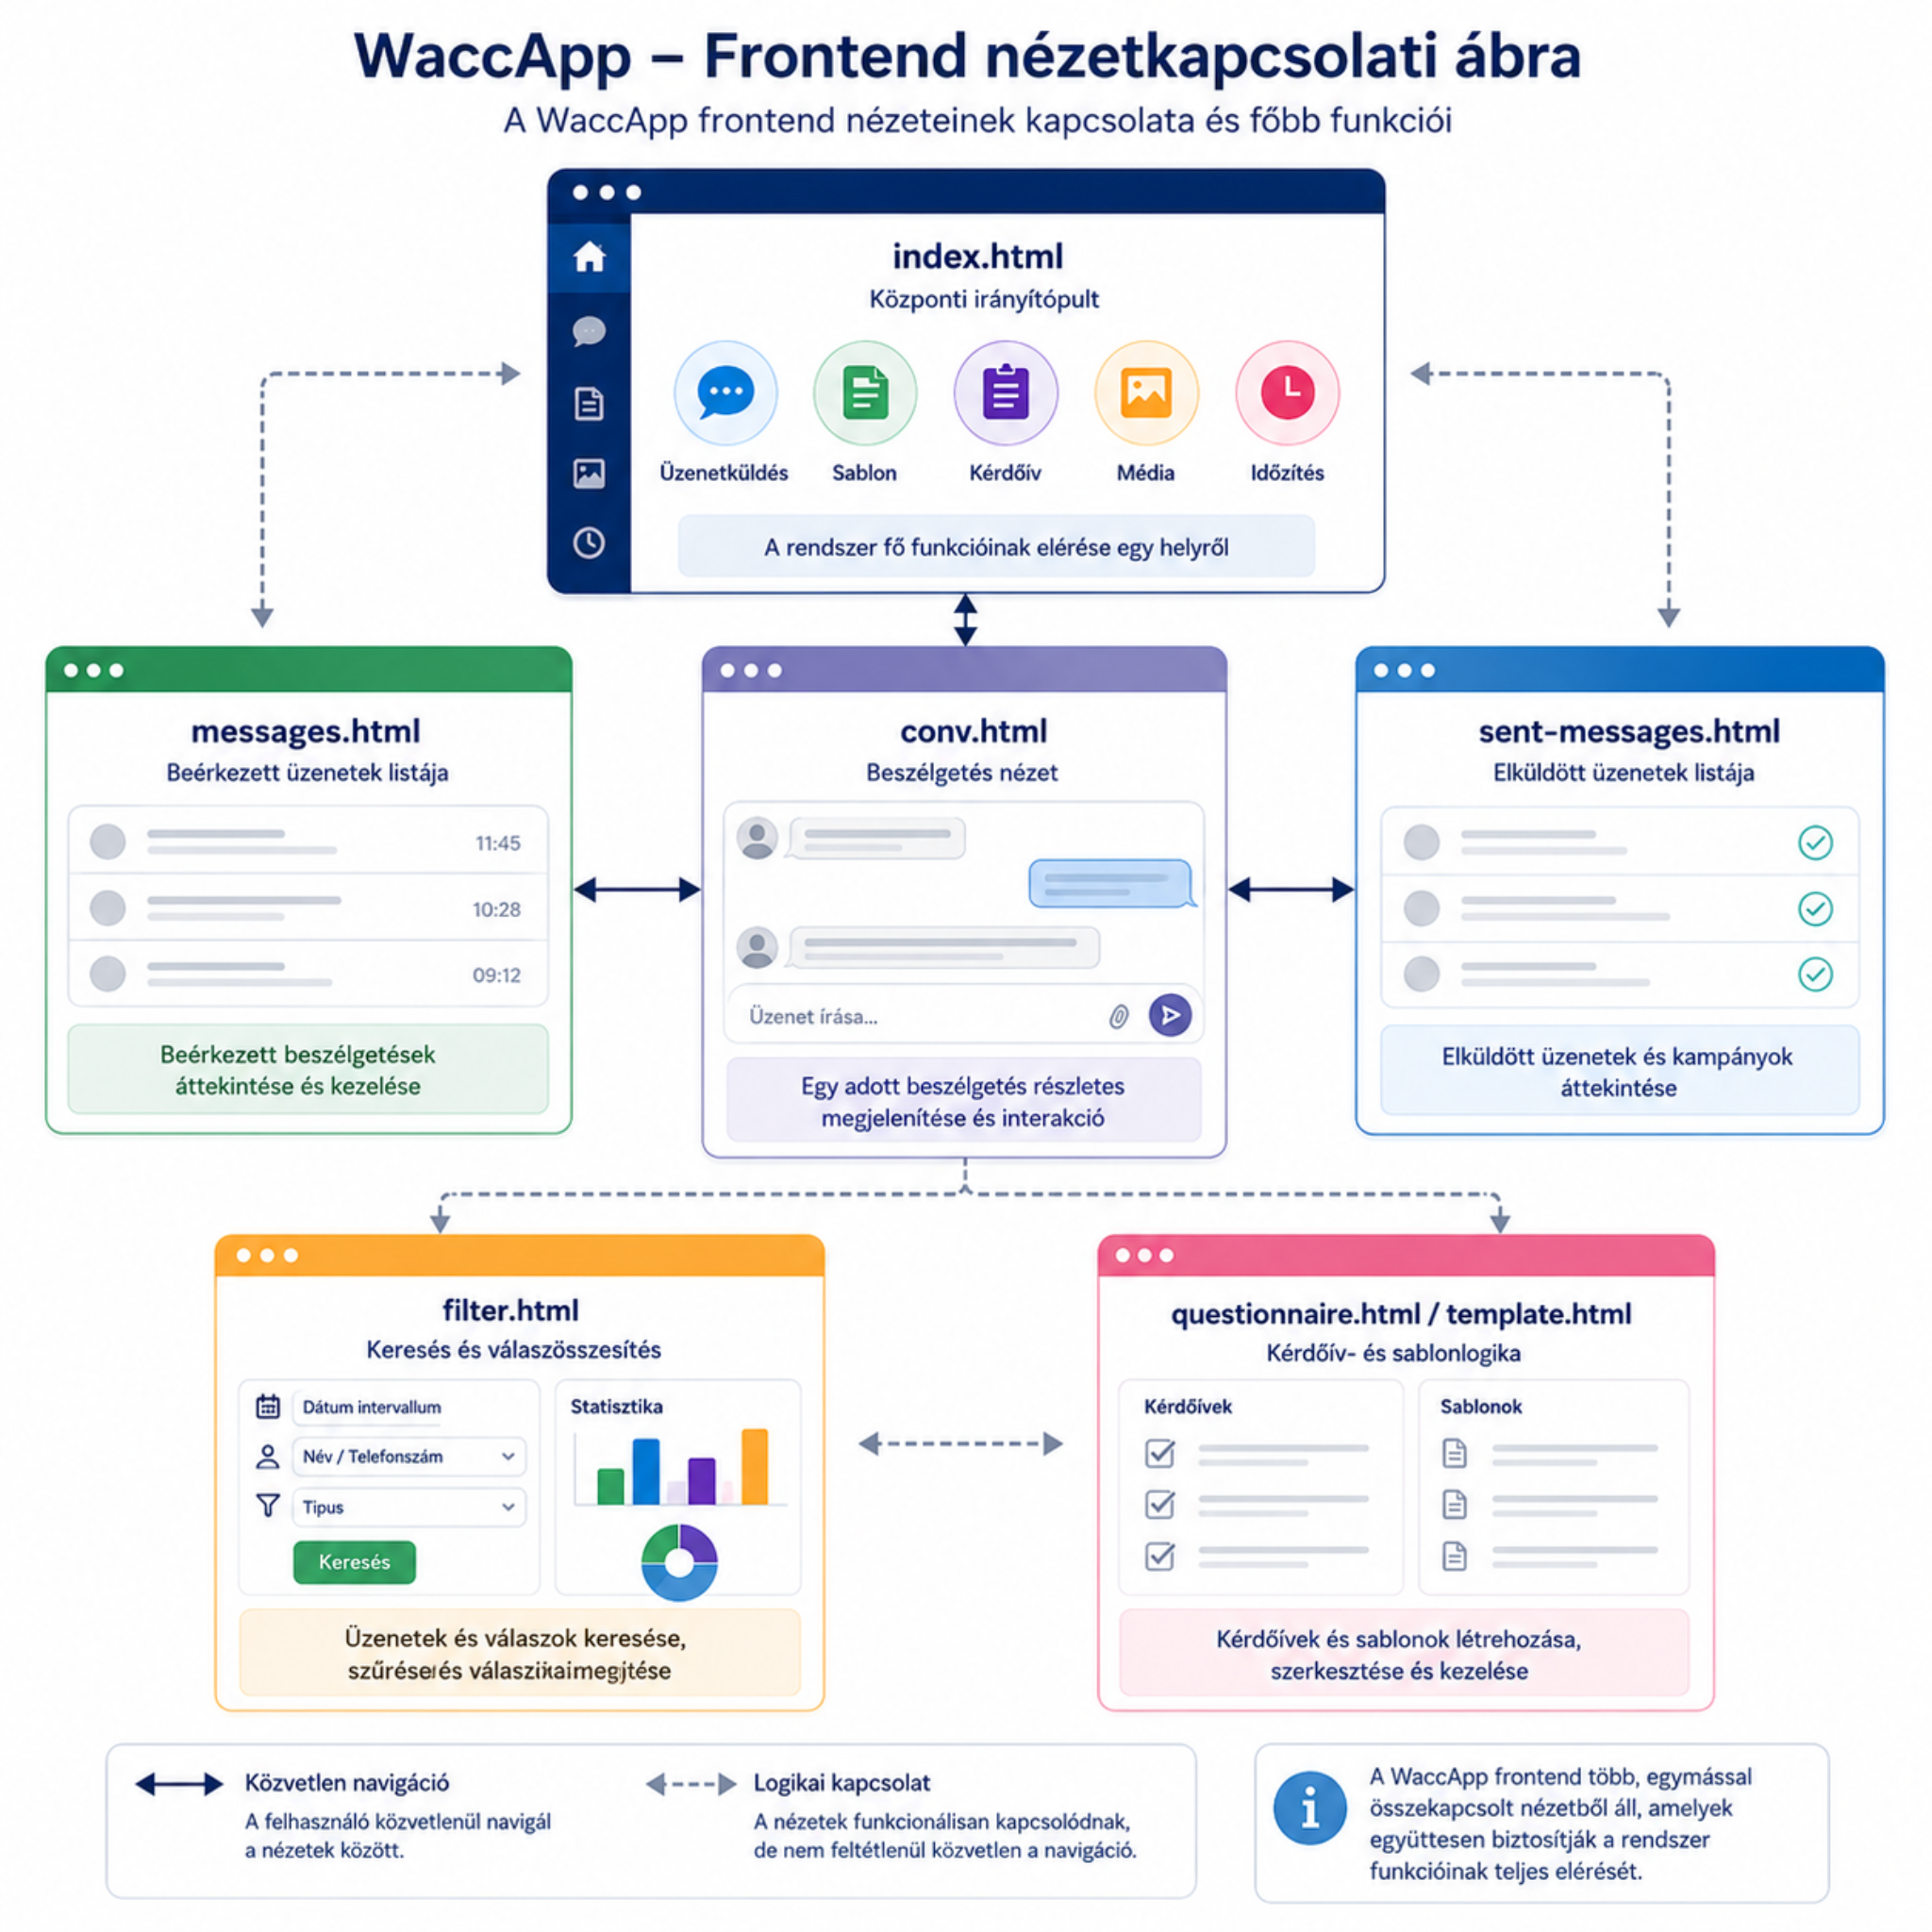
\includegraphics[width=0.95\textwidth]{images/waccapp-frontend-nezetkapcsolat.png}
\caption{A WaccApp frontend nézeteinek kapcsolata és főbb funkciói.}
\label{fig:frontend-nezetkapcsolat}
\end{figure}

Az ábrán elkülönülnek azok a nézetek, amelyek közvetlen felhasználói navigációval érhetők el, és azok a kapcsolatok, amelyek inkább funkcionális összefüggést jelentenek. Az \path{index.html} a kommunikációs műveletek indítófelülete, a \path{messages.html} és a \path{sent-messages.html} a kommunikációs események listaalapú áttekintését segítik, a \path{conv.html} pedig egy adott beszélgetés részletesebb értelmezését biztosítja. A \path{filter.html} ehhez képest a létrejött adatok visszakeresését és egyszerű válaszösszesítését támogatja. A \path{questionnaire.html} és a \path{template.html} a kérdőíves és sablonos logika előkészítéséhez kapcsolódik. Az ábra ezzel azt szemlélteti, hogy a WaccApp frontendje nem elszigetelt oldalakból áll, hanem egymásra épülő nézetek rendszeréből.

\section{A frontend mappaszerkezete és fő fájljai}

A WaccApp frontendjének mappaszerkezete a rendszer funkcionális felépítését követi. A nyilvánosan elérhető kliensoldali állományok a public könyvtárban találhatók. Ebben a mappában helyezkednek el azok a HTML-fájlok, amelyek a felhasználó által közvetlenül elérhető nézeteket adják. A struktúra előnye, hogy a frontend fő oldalai egy helyen, áttekinthető módon kapcsolódnak a backend által kiszolgált webes környezethez. 

A public mappában található központi kommunikációs felület az \path{index.html}, amelyhez a küldési műveletek jelentős része kapcsolódik. Ugyanitt találhatók a kommunikációs előzményekhez tartozó nézetek, például a \path{messages.html}, a \path{sent-messages.html} és a \path{conv.html}. A szűréshez és visszakereséshez a \path{filter.html} kapcsolódik, míg a kérdőíves és sablonos szerkesztési feladatokhoz a \path{questionnaire.html}, a \path{template.html}, a \path{template-menu.html} és a \path{template-single.html} tartozik. A \path{login.html}, a \path{menu.html}, az \path{admin.html}, az \path{account.html} és a \path{privacy.html} a rendszer használatának kiegészítő, navigációs vagy tájékoztató elemeit adják. 

A médiaelemek kezeléséhez két fontos mappa kapcsolódik. A public/uploads a feltöltött vagy előkészített állományokhoz kötődik, míg a public/sent\_media az elküldött médiafájlok visszakövethető megjelenítésében kap szerepet. Ez a szétválasztás azért fontos, mert a médiakezelés nemcsak fájltechnikai kérdés, hanem a beszélgetésnézet és a kommunikációs előzmények értelmezhetőségének része is. Ha egy elküldött kép vagy dokumentum később a \path{conv.html} felületen is megjelenik, akkor a felhasználó nem pusztán az állomány létezését látja, hanem azt is, hogy az melyik kommunikációs folyamatba illeszkedett. 

A frontend működéséhez szorosan kapcsolódik a gyökérszinten található \path{questionnaire.js}, amely a kérdőíves logikák egyik fontos adatszerkezeti hátterét adja. Ebben jelennek meg azok a kérdőívfolyamatok, amelyekhez a frontend szerkesztő- és indítófelületei kapcsolódhatnak. Az app.js szerveroldali fájl, de a frontend működésének megértéséhez elengedhetetlen, mert ebben találhatók azok a végpontok, amelyeket a kliensoldali nézetek meghívnak. Az \path{app.js} nem backendimplementációként kerül részletes elemzésre, hanem kapcsolódási pontként. A teljes, frontend szempontból releváns mappaszerkezet a 15.1. mellékletben található.

\section{A szerkezet előnyei és korlátai}

A WaccApp frontendarchitektúrájának egyik legfontosabb előnye, hogy a különböző funkciók világos felelősségi köröket kapnak. Az \path{index.html} a küldési műveletekre koncentrál, a \path{conv.html} a beszélgetések értelmezésére, a \path{filter.html} a visszakeresésre és alapvető elemzésre, a \path{questionnaire.html} és a sablonkezelő oldalak pedig a kérdőíves folyamatok létrehozására. Ez a felosztás megkönnyíti annak megértését, hogy egy adott funkció hol található, és fejlesztői oldalról is egyszerűbbé teszi a hibák lokalizálását. 

A szerkezet előnye a fokozatos bővíthetőség is. Ha a rendszer később új kommunikációs funkcióval, fejlettebb statisztikai nézettel vagy részletesebb adminisztratív felülettel bővülne, az új elem önálló nézetként vagy egy meglévő oldal célzott kiegészítéseként is bevezethető lenne. Ez a projekt jelenlegi méretéhez és céljához jól illeszkedik, mert nem kényszeríti a rendszert túlzottan összetett frontend-keretrendszer használatára, ugyanakkor megőrzi a funkciók elkülöníthetőségét. 

A szerkezetnek ugyanakkor korlátai is vannak. Mivel a rendszer nem egy központi kliensoldali keretrendszerre épül, az egységes működés nem automatikusan következik a technológiából. A hasonló gombhasználatot, állapotjelzést, validációt és felületi viselkedést fejlesztési döntésekkel kellett fenntartani. Ez nagyobb odafigyelést igényel, mert ha az egyes HTML-oldalak eltérő logikát kezdenének követni, a rendszer könnyen széttartóvá válhatna. 

További korlát, hogy egy nagyobb, valós idejű működésre vagy összetett globális állapotkezelésre épülő rendszer esetében egy modern frontend keretrendszer előnyösebb lehetne. Egy React-, Vue- vagy Angular-alapú alkalmazás például központosítottabb állapotkezelést és újrahasznosítható komponensrendszert biztosíthatna. Ezért a keretrendszeres megvalósítás nem elvetett, hanem későbbi továbbfejlesztési irányként értelmezhető. A WaccApp jelenlegi célrendszerében azonban a több HTML-nézetből álló szerkezet védhető döntés, mert a rendszer fő feladatai jól elkülöníthetők és a fejlesztés áttekinthető marad. 

\section{A szerkezeti döntések szerepe a modulok bemutatásában}

A WaccApp frontendjének szerkezeti döntései közvetlenül előkészítik a kiemelt modulok részletes bemutatását. A többnézetes architektúra azért fontos, mert a következő fejezetben tárgyalt funkciók már nem elméleti követelményként, hanem konkrét oldalakhoz és felhasználói folyamatokhoz kötve jelennek meg. Az üzenetküldés az \path{index.html} felületből indul, a beszélgetések értelmezését a \path{conv.html} támogatja, a visszakeresést a \path{filter.html} biztosítja, a kérdőíves működés a \path{questionnaire.html} és a sablonkezelő oldalak köré szerveződik, a médiafájlok pedig a uploads és sent\_media mappákon keresztül válnak a felület részévé. 

A WaccApp megértéséhez nem elegendő az egyes funkciókat külön-külön bemutatni. Előbb látni kell azt a szerkezetet, amelyben ezek a funkciók elhelyezkednek. A frontend architektúrája adja meg azt az alaprajzot, amelyre a modulok részletes működése ráépül. A WaccApp frontendje tehát nem véletlenszerű HTML-fájlokból összeálló felület, hanem olyan többnézetes rendszer, amelyben az egyes oldalak saját felelősséget kapnak, mégis közös kommunikációs cél mentén kapcsolódnak össze. Ez az architekturális alap teszi lehetővé, hogy a dolgozat következő része már a rendszer kiemelt moduljait, azok működését és saját frontendmegoldásait részletesen tárgyalja. [R10], [R13] 
